\chead{\ifthenelse{\value{page}=1}{}{\textit{Species interactions in Markov networks}}}
\renewcommand{\headrulewidth}{0pt}

\setlength{\parskip}{3pt}

\textbf{Title:} Estimating species interactions from observational data
with Markov networks

\textbf{Author:} David J. Harris: Population Biology; 1 Shields Avenue,
Davis CA, 95616

\textbf{Abstract:} Estimating species interactions from observational
data is one of the most controversial tasks in community ecology. One
difficulty is that a single pairwise interaction can ripple through an
ecological network and produce surprising indirect consequences. For
example, the negative correlation between two competing species can be
reversed in the presence of a third species that is capable of
outcompeting both of them. Here, I apply models from statistical
physics, called Markov networks or Markov random fields, that can
predict the direct and indirect consequences of any possible species
interaction matrix. Interactions in these models can be estimated from
observational data via maximum likelihood. Using simulated landscapes
with known pairwise interaction strengths, I evaluated Markov networks
and six existing approaches. The Markov networks consistently
outperformed other methods, correctly isolating direct interactions
between species pairs even when indirect interactions largely
overpowered them. Two computationally efficient approximations, based on
linear and generalized linear models, also performed well. Indirect
effects reliably caused a common null modeling approach to produce
incorrect inferences, however.

\textbf{Key words:} Ecological interactions; Occurrence data; Species
associations; Markov network; Markov random field; Ising model;
Biogeography; Presence--absence matrix; Null model

\subsubsection{Introduction}\label{introduction}

\setlength{\parindent}{1cm}

To the extent that nontrophic species interactions (such as competition)
affect community assembly, ecologists might expect to find signatures of
these interactions in species composition data
\citep{macarthur_population_1958, diamond_island_1975}. Despite decades
of work and several major controversies, however
\citep{lewin_santa_1983, strong_ecological_1984, gotelli_swap_2003, connor_checkered_2013},
existing methods for detecting competition's effects on community
structure are unreliable \citep{gotelli_empirical_2009}. In particular,
species' effects on one another can become lost in the complex web of
direct and indirect interactions in real assemblages. For example, the
competitive interaction between the two shrub species in Figure 1A can
become obscured by their shared tendency to occur in unshaded areas
(Figure 1B). While ecologists have long known that indirect effects can
overwhelm direct ones at the landscape level
\citep{dodson_complementary_1970, levine_competitive_1976}, the vast
majority of our methods for drawing inferenes from observational data do
not control for these effects
\citep[e.g.][]{diamond_island_1975, strong_ecological_1984, gotelli_empirical_2009, veech_probabilistic_2013, pollock_understanding_2014}.
To the extent that indirect interactions like those in Figure 1 are
generally important \citep{dodson_complementary_1970}, existing methods
will thus not generally provide much evidence regarding species' direct
effects on one another. The goal of this paper is to resolve this
long-standing problem.

\begin{figure}[htbp]
\centering
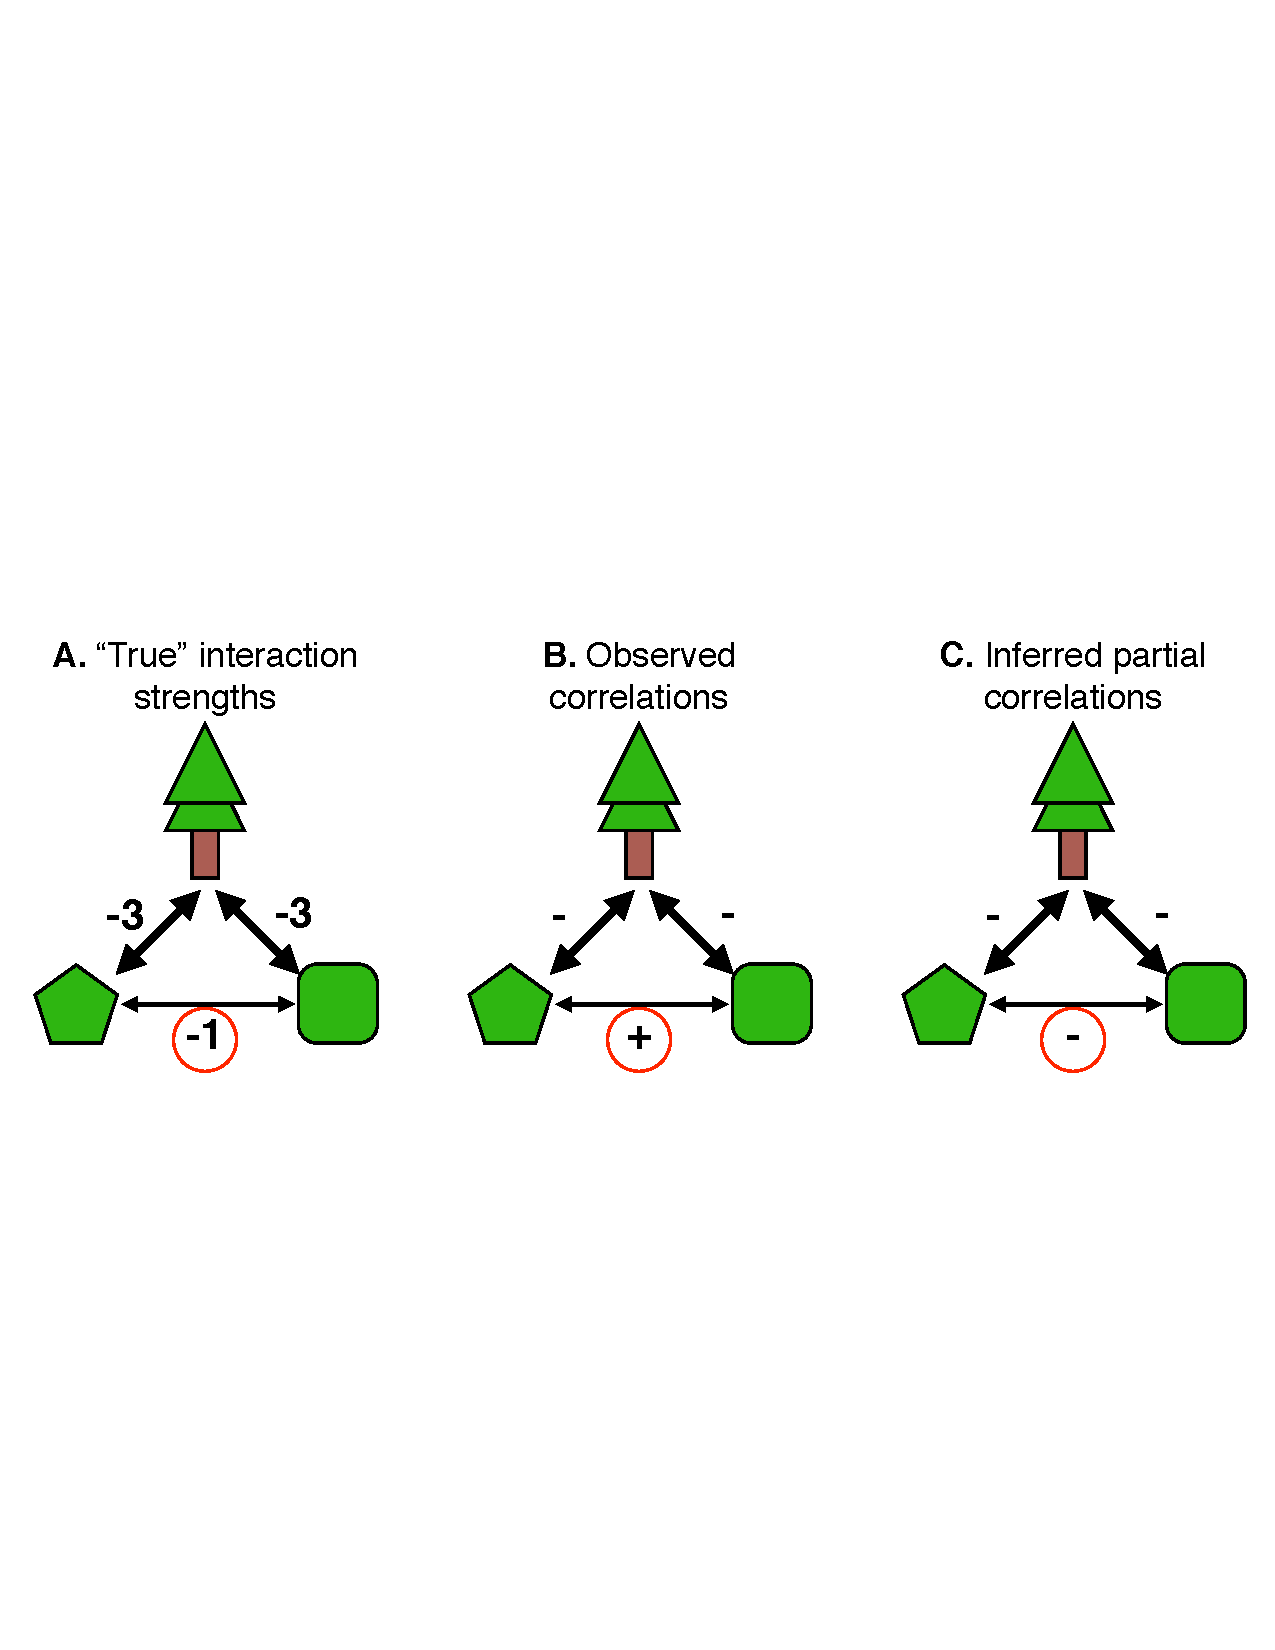
\includegraphics{figures/Figure_1.pdf}
\caption{\textbf{Figure 1.} \textbf{A.} A small network of three
competing species. The tree (top) tends not to co-occur with either of
the two shrub species, as indicated by the strongly negative coefficient
linking them. The two shrub species also compete with one another, but
more weakly (circled coefficient). \textbf{B.} In spite of the
competitive interactions between the two shrub species, their shared
tendency to occur in locations without trees makes their occurrence
vectors positively correlated (circled). \textbf{C.} Controlling for the
tree species' presence with a conditional method such as a partial
covariance or a Markov network leads to correct identification of the
negative shrub-shrub interaction (circled).}
\end{figure}

While competition doesn't reliably reduce co-occurrence rates at the
whole-landscape level (as most of our methods assume), it nevertheless
does leave a signal in the data (Figure 1C). Specifically, after
partitioning the data set into shaded sites and unshaded sites, there
will be co-occurrence deficits in each subset that might not be apparent
at the landscape level. More generally, we can obtain much better
estimates of the association between two species from their conditional
relationships (i.e.~by controlling for other species in the network)
than we could get from their overall co-occurrence rates. This kind of
precision is difficult to obtain from null models, which begin with the
assumption that all the pairwise interactions are zero and thus don't
need to be controlled for. Nevertheless, null models have dominated this
field for more than three decades
\citep{strong_ecological_1984, gotelli_empirical_2009}.

Following recent work by \citet{azaele_inferring_2010} and
\citet{fort_statistical_2013}, this paper shows that Markov networks
\citep[undirected graphical models also known as Markov random
fields;][]{murphy_machine_2012} can provide a framework for
understanding the landscape-level consequences of pairwise species
interactions, and for detecting them from observed presence-absence
matrices. Markov networks have been used in many scientific fields in
similar contexts for decades, from physics \citep[where nearby particles
interact magnetically;][]{cipra_introduction_1987} to spatial statistics
\citep[where adjacent grid cells have correlated
values;][]{harris_contact_1974, gelfand_modelling_2005}. While community
ecologists explored some related approaches in the 1980's
\citep{whittam_species_1981}, they used severe approximations that led
to unintelligible results \citep[e.g. ``probabilities'' greater than
one;][]{gilpin_factors_1982}.

Below, I introduce Markov networks and show how they can be used to
simulate landscape-level data or to make exact predictions about the
direct and indirect consequences of possible interaction matrices. Then,
using simulated data sets where the ``true'' interactions are known, I
compare this approach with several existing methods. Finally, I discuss
opportunities for extending the approach presented here to other
problems in community ecology, e.g.~quantifying the overall effect of
species interactions on occurrence rates
\citep{roughgarden_competition_1983} and disentangling the effects of
biotic versus abiotic interactions on species composition
\citep{kissling_towards_2012, pollock_understanding_2014}.

\subsubsection{Methods}\label{methods}

\paragraph{Markov networks.}\label{markov-networks.}

Markov networks provide a framework for translating back and forth
between the conditional relationships among species (Figure 1C) and the
kinds of species assemblages that these relationships produce. Here, I
show how a set of conditional relationships can be used to determine how
groups of species can co-occur. Methods for estimating conditional
relationships from data are discussed in the next section.

A Markov network defines the relative probability of observing a given
vector of species-level presences (1s) and absences (0s), \(\vec{y}\),
as

\centering

\(p(\vec{y}; \alpha, \beta) \propto exp(\sum_{i}\alpha_i y_i + \sum_{i\neq j}\beta_{ij}y_i y_j).\)

\raggedright
\setlength{\parindent}{1cm}

Here, \(\alpha_{i}\) is an intercept term determining the amount that
the presence of species \(i\) contributes to the log-probability of
\(\vec{y}\); it directly controls the prevalence of species \(i\).
Similarly, \(\beta_{ij}\) is the amount that the co-occurrence of
species \(i\) and species \(j\) contributes to the log-probability; it
controls the conditional relationship between two species, i.e.~the
probability that they will be found together, after controlling for the
other species in the network (Figure 2A, Figure 2B). For example,
\(\beta_{ij}\) might have a value of \(+2\) for two mutualists,
indicating that the odds of observing one species are \(e^2\) times
higher in sites where its partner is present than in comparable sites
where its partner is absent. Because the relative probability of a
presence-absence vector increases when positively-associated species
co-occur and decreases when negatively-associated species co-occur, the
model tends---all else equal---to produce assemblages that have many
pairs of positively-associated species and relatively few pairs of
negatively-associated species (exactly as an ecologist might expect).

\begin{figure}[htbp]
\centering
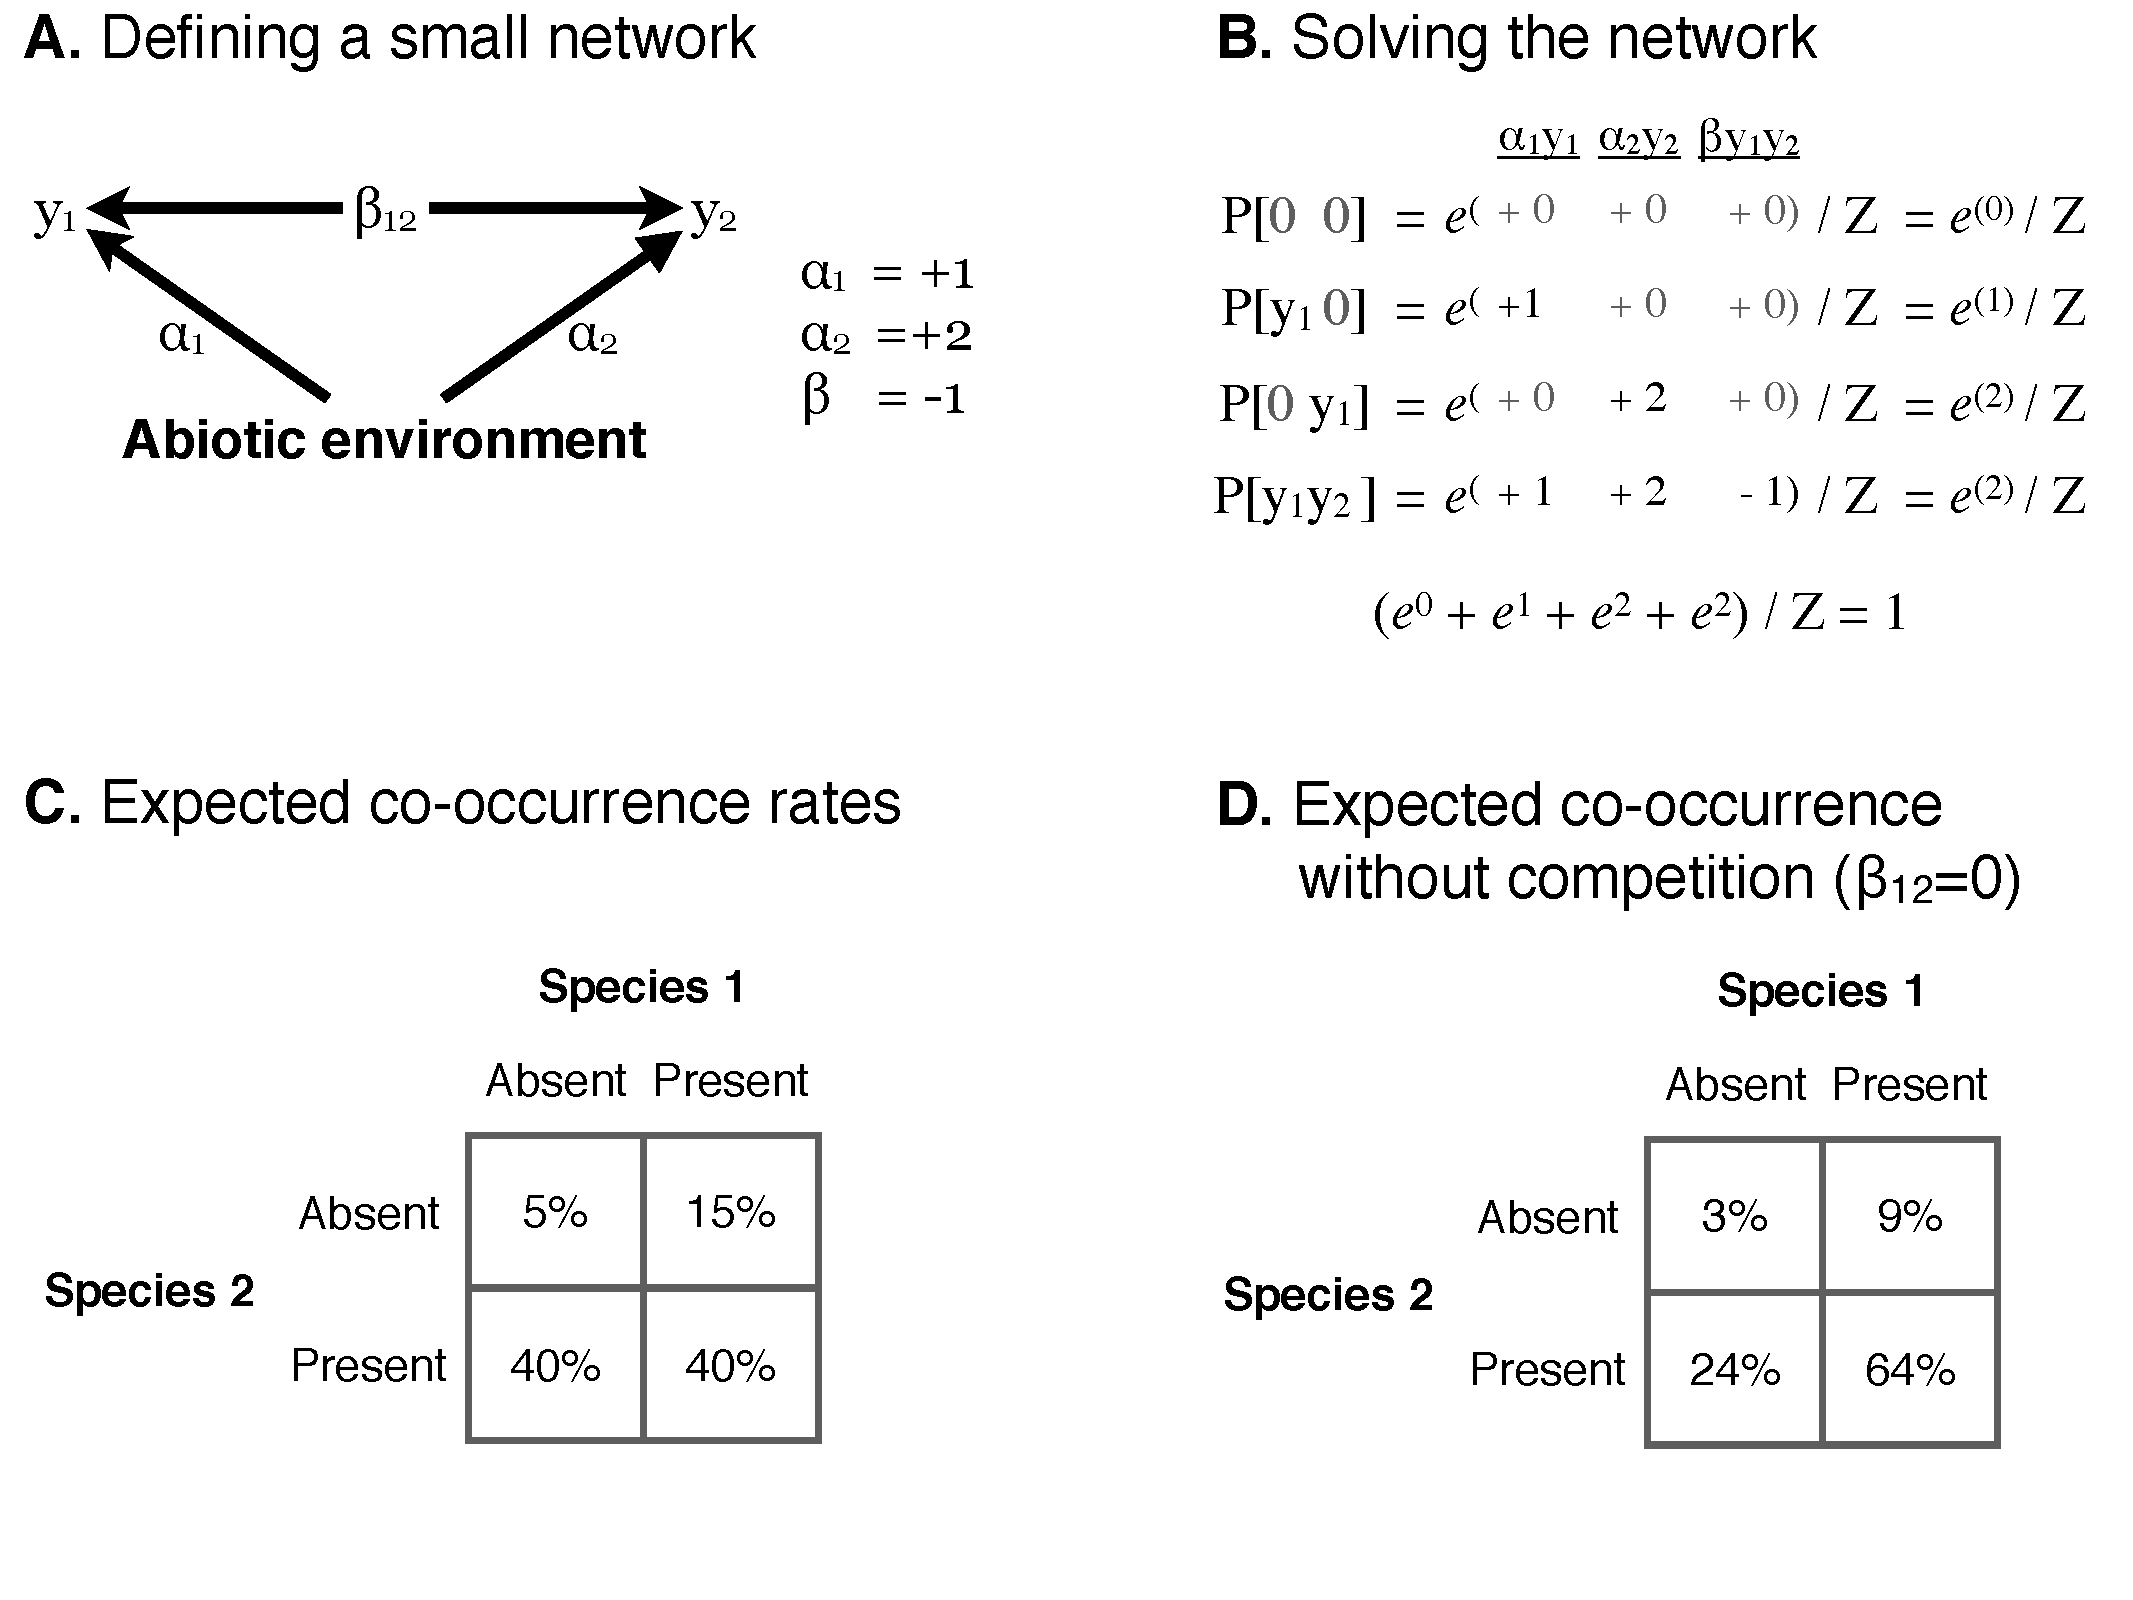
\includegraphics{figures/Figure_2.pdf}
\caption{\textbf{Figure 2.} \textbf{A.} A small Markov network with two
species. The abiotic environment favors the occurrence of both species
(\(\alpha >0\)), particularly species 2 (\(\alpha_2 > \alpha_1\)). The
negative \(\beta\) coefficient linking these two species implies that
they co-occur less than expected under independence. \textbf{B.}
Relative probabilities of all four possible presence-absence
combinations for Species 1 and Species 2. The exponent includes
\(\alpha_1\) whenever Species 1 is present (\(y_1 = 1\)), but not when
it is absent (\(y_1 = 0\)). Similarly, the exponent includes
\(\alpha_2\) only when species \(2\) is present (\(y_2 = 1\)), and
\(\beta\) only when both are present (\(y_1y_2 = 1\)). The normalizing
constant \(Z\), ensures that the four relative probabilities sum to 1.
In this case, \(Z\) is about 18.5. \textbf{C.} We can find the expected
frequencies of all possible co-occurrence patterns between the two
species of interest. \textbf{D.} If \(\beta_{12}\) equaled zero (e.g.~if
the species no longer competed for the same resources), then the
reduction in competition would allow each species to increase its
occurrence rate and the co-occurrence deficit would be eliminated.}
\end{figure}

Of course, if all else is \emph{not} equal (e.g.~Figure 1, where the
presence of one competitor is associated with release from another
competitor), then species' marginal association rates can differ from
this expectation. Determining the marginal relationships between species
from their conditional interactions entails summing over the different
possible assemblages (Figure 2B). This becomes intractable when the
number of possible assemblages is large, though several methods beyond
the scope of this paper can be employed to keep the calculations
feasible \citep{lee_learning_2012, salakhutdinov_learning_2008}.
Alternatively, as noted below, some common linear and generalized linear
methods can also be used as computationally efficient approximations to
the full network \citep{lee_learning_2012, loh_structure_2013}.

\paragraph{\texorpdfstring{Estimating \(\alpha\) and \(\beta\)
coefficients from presence-absence
data.}{Estimating \textbackslash{}alpha and \textbackslash{}beta coefficients from presence-absence data.}}\label{estimating-alpha-and-beta-coefficients-from-presence-absence-data.}

In the previous section, the values of \(\alpha\) and \(\beta\) were
known and the goal was to make predictions about possible species
assemblages. In practice, however, ecologists will often need to
estimate the parameters from an observed co-occurrence matrix (i.e.~from
a matrix of ones and zeros indicating which species are present at which
sites). When the number of species is reasonably small, one can compute
exact maximum likelihood estimates for all of the \(\alpha\) and
\(\beta\) coefficients given a presence-absence matrix by optimizing
\(p(\vec{y}; \alpha, \beta)\). Fully-observed Markov networks like the
ones considered here have unimodal likelihood surfaces
\citep{murphy_machine_2012}, ensuring that this procedure will always
converge on the global maximum. This maximum represents the unique
combination of \(\alpha\) and \(\beta\) coefficients that would be
expected to produce exactly the observed co-occurrence frequencies on
average \citep[i.e.~maximizing the likelihood matches the sufficient
statistics of the model distribution to the sufficient statistics of the
data;][]{murphy_machine_2012}. I used the rosalia package
\citep{harris_rosalia_2015} for the R programming language
\citep{r_core_team_r_2015} to optimize the Markov network parameters.
The package was named after Santa Rosalia, the patron saint of
biodiversity, whose supposedly miraculous healing powers played an
important rhetorical role in the null model debates of the 1970's and
1980's \citep{lewin_santa_1983}.

\paragraph{Simulated landscapes.}\label{simulated-landscapes.}

In order to compare different methods, I simulated two sets of
landscapes using known parameters. The first set included the three
competing species shown in Figure 1. For each of 1000 replicates, I
generated a landscape with 100 sites by sampling from a probability
distribution defined by the figure's interaction coefficients (Appendix
1). Each of the methods described below was then evaluated on its
ability to correctly infer that the two shrub species competed with one
another, despite their frequent co-occurrence.

I also simulated a second set of landscapes using a stochastic community
model based on generalized Lotka-Volterra dynamics, as described in
Appendix 2. In these simulations, each species pair was randomly
assigned to either compete for a portion of the available carrying
capacity (negative interaction) or to act as mutualists (positive
interaction). Here, mutualisms operate by mitigating the effects of
intraspecific competition on each partner's death rate. For these
analyses, I simulated landscapes with up to 20 species and 25, 200, or
1600 sites (50 replicates per landscape size; see Appendix 2).

\paragraph{Recovering species interactions from simulated
data.}\label{recovering-species-interactions-from-simulated-data.}

I compared seven techniques for determining the sign and strength of the
associations between pairs of species from simulated data (Appendix 3).
First, I used the rosalia package \citep{harris_rosalia_2015} to fit
Markov newtork models, as described above. For the analyses with 20
species, I added a very weak logistic prior distribution on the
\(\alpha\) and \(\beta\) terms with scale 2 to ensure that the model
estimates were always finite. The bias introduced by this prior should
be small: the 95\% credible interval on \(\beta\) only requires that one
species' effect on the odds of observing a different species to be less
than a factor of 1500 (which is not much of a constraint). The logistic
distribution was chosen because it is convex and has a similar shape to
the Laplace distribution used in LASSO regularization (especially in the
tails), but unlike the Laplace distribution it is differentiable
everywhere and does not force any estimates to be exactly zero. To
confirm that this procedure produced stable estimates, I compared its
estimates on 50 bootstrap replicates (Appendix 4).

I also evaluated six alternative methods: five from the existing
literature, plus a novel combination of two of these methods. The first
alternative interaction metric was the sample correlation between
species' presence-absence vectors, which summarizes their marginal
association. Next, I used partial correlations, which summarize species'
conditional relationships
\citep{albrecht_spatial_2001, faisal_inferring_2010}. In the context of
non-Gaussian data, the partial correlation can be thought of as a
computationally efficient approximation to the full Markov network model
\citep{loh_structure_2013}. This sort of model is very common for
estimating relationships among genes and gene products
\citep{friedman_sparse_2008}. Because partial correlations are undefined
for landscapes with perfectly-correlated species pairs, I used a
regularized estimate based on James-Stein shrinkage, as implemented in
the corpcor package's \texttt{pcor.shrink} function with the default
settings \citep{schafer_corpcor_2014}.

The third alternative, generalized linear models (GLMs), can also be
thought of as a computationally efficient approximation to the Markov
network \citep{lee_learning_2012}. Following
\citet{faisal_inferring_2010}, I fit regularized logistic regression
models \citep{gelman_weakly_2008} for each species, using the other
species on the landscape as predictors. To avoid the identifiability
problems associated with directed cyclic graphs
\citep{schmidt_modeling_2012}, I then symmetrized the relationships
within species pairs via averaging.

The next method, described in \citet{gotelli_empirical_2009}, involved
simulating new landscapes from a null model that retains the row and
column sums of the original matrix \citep{strong_ecological_1984}. I
used the \(Z\)-scores computed by the Pairs software described in
\citet{gotelli_empirical_2009} as my null model-based estimator of
species interactions.

The last two estimators used the latent correlation matrix estimated by
the BayesComm package \citep{golding_bayescomm_2015} in order to
evaluate the recent claim that the correlation coefficients estimated by
``joint species distribution models'' provide an accurate assessment of
species' pairwise interactions
\citetext{\citealp{pollock_understanding_2014}; \citealp[see
also][]{harris_generating_2015}}. In addition to using the posterior
mean correlation \citep{pollock_understanding_2014}, I also used the
posterior mean \emph{partial} correlation, which might be able to
control for indirect effects.

\paragraph{Evaluating model
performance.}\label{evaluating-model-performance.}

For the simulated landscapes based on Figure 1, I assessed whether each
method's test statistic indicated a positive or negative relationship
between the two shrubs (Appendix 1). For the null model (Pairs), I
calculated statistical significance using its \(Z\)-score. For the
Markov network, I used the Hessian matrix to generate approximate
confidence intervals and noted whether these intervals included zero.

I then evaluated the relationship between each method's estimates and
the ``true'' interaction strengths among all of the species pairs from
the larger simulated landscapes. This determined which of the methods
provide a consistent way to know how strong species interactions
are---regardless of which species were present in a particular data set
or how many observations were taken. Because the different methods
mostly describe species interactions on different scales
(e.g.~correlations versus \(Z\) scores versus regression coefficients),
I used linear regression through the origin to rescale the different
estimates produced by each method so that they had a consistent
interpretation. After rescaling each method's estimates, I calculated
squared errors between the scaled interaction estimates and ``true''
interaction values across all the simulated data sets. These squared
errors determined the proportion of variance explained for different
combinations of model type and landscape size (compared with a null
model that assumed all interaction strengths to be zero).

\subsubsection{Results}\label{results}

\paragraph{Three species.}\label{three-species.}

As shown in Figure 1, the marginal relationship between the two shrub
species was positive---despite their competition for space at a
mechanistic level---due to indirect effects of the dominant tree
species. As a result, the correlation between these species was positive
in 94\% of replicates, and the randomization-based null model falsely
reported positive associations 100\% of the time. Worse, more than 98\%
of these false conclusions were statistically significant. The partial
correlation and Markov network estimates, on the other hand, each
correctly isolated the direct negative interaction between the shrubs
from their positive indirect interaction 94\% of the time (although the
confidence intervals overlapped zero in most replicates).

\paragraph{Twenty species.}\label{twenty-species.}

Despite some variability across contexts (Figure 3A), the four methods
that controlled for indirect effects clearly performed the best: the
Markov network explained the largest portion of the variance in the
``true'' interaction coefficients (35\% overall), followed by the
generalized linear models (30\%), partial correlations from the raw
presence-absence data (28\%), and partial correlations from BayesComm,
the joint species distribution model (26\%). The benefit of choosing the
full Markov network over the other three methods was largest on the
smaller landscapes, which are also the ones that are most representative
of typical analyses in this field \citep{gotelli_empirical_2009}.

\begin{figure}[htbp]
\centering
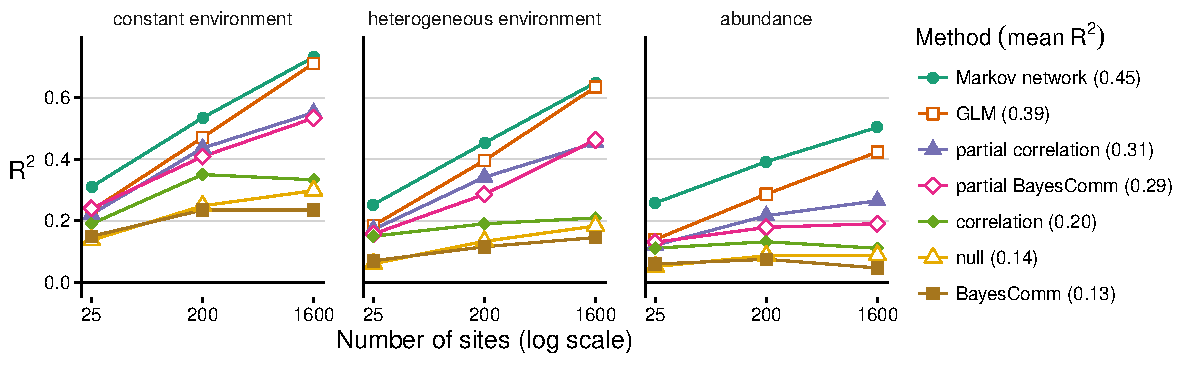
\includegraphics{figures/performance.pdf}
\caption{\textbf{Figure 3.} \textbf{A.} Proportion of variance in
interaction coefficients explained by each method versus number of
sampled locations. \textbf{B.} The \(Z\)-scores produced by the null
model (``Pairs'') for each pair of species can be predicted using the
correlation between the presence-absence vectors of those same species
and from the number of sites on the landscape.}
\end{figure}

The three methods that did not attempt to control for indirect
interactions all explained less than 20\% of the variance. Of these, the
sample correlation matrix based on the raw data performed the best
(19\%), followed by the null model (15\%) and BayesComm's correlation
matrix (11\%). Although these last three methods had different \(R^2\)
values, there was a close mapping among their estimates (especially
after controlling for the size of the simulated landscapes; Figure 3B).
This suggests that the effect sizes from the null model (and, to a
lesser extent, the correlation matrices from joint species distribution
models) only contain noisy versions of the same information that could
be obtained more easily and interpretably by calculating correlation
coefficients between species' presence-absence vectors.

Bootstrap resampling indicated that the above ranking of the different
methods was robust (Appendix 3). In particular, the 95\% confidence
interval of the bootstrap distribution indicated that the Markov
network's overall \(R^2\) value was between 14 and 18 percent higher
than the second-most effective method (generalized linear models) and
between 2.12 and 2.38 times higher than could be achieved by the null
model (Pairs). Bootstrap resampling of a 200-site landscape also
confirmed that the rosalia package's estimates of species' conditional
relationships were robust to sampling variation for reasonably-sized
landscapes (Appendix 4).

\subsubsection{Discussion}\label{discussion}

The results presented above show that Markov networks can reliably
recover species' pairwise interactions from observational data, even for
cases where a common null modeling technique reliably fails.
Specifically, Markov networks were successful even when direct
interactions were largely overwhelmed by indirect effects (Figure 1).
For cases where fitting a Markov network is computationally infeasible,
these results also indicate that partial covariances and generalized
linear models (the two methods that estimated conditional relationships
rather than marginal ones) can both provide useful approximations. The
partial correlations' success on simulated data may not carry over to
real data sets, however; \citet{loh_structure_2013} show that the linear
approximations can be less reliable in cases where the true interaction
matrix contains more structure (e.g.~guilds or trophic levels).
Similarly, the approximation involved in using separate generalized
linear models for each species can occasionally lead to catastrophic
overfitting with small-to-moderate sample sizes
\citep{lee_learning_2012}. For these reasons, it will usually be best to
fit a Markov network rather than one of the alternative methods when
one's computational resources allow it.

It's important to note that none of these methods can identify the exact
nature of the pairwise interactions \citep[e.g.~which species in a
positively-associated pair is facilitating the
other;][]{schmidt_modeling_2012}, particularly when real pairs of
species can reciprocally influence one another in multiple ways
simultaneously \citep{bruno_inclusion_2003}; with compositional data,
there is only enough information to provide a single number describing
each species pair. To estimate asymmetric interactions, such as
commensalism or predation, ecologists would need other kinds of data, as
from time series, behavioral observations, manipulative experiments, or
natural history. These other sources of information could also be used
to augment the likelihood function with an informative prior
distribution, which could lead to better results on some real data sets
than was shown in Figure 3A.

Despite their limitations, Markov networks have enormous potential to
improve ecological understanding. In particular, they are less
vulnerable than some of the most commonly-used methods to mistakenly
identifying positive species interactions between competing species, and
can make precise statements about the conditions where indirect
interactions will overwhelm direct ones. They also provide a simple
answer to the question of how competition should affect a species'
overall prevalence, which was a major flashpoint for the null model
debates in the 1980's
\citep{roughgarden_competition_1983, strong_ecological_1984}. Equation 1
can be used to calculate the expected prevalence of a species in the
absence of biotic influences
\citep[\(\frac{e^\alpha}{1 + e^{\alpha}}\);][]{lee_learning_2012}.
Competition's effect on prevalence in a Markov network can then be
calculated by subtracting this value from the observed prevalence (cf
Figure 2D). This kind of insight would have been difficult to obtain
without a generative model that makes predictions about the consequences
of species interactions; null models (which presume \emph{a priori} that
interactions do not exist) have no way to make such predictions.

Markov networks---particularly the Ising model for binary
networks---have been studied for nearly a century
\citep{cipra_introduction_1987}, and the models' properties,
capabilities, and limits are well-understood in a huge range of
applications. Using the same framework for species interactions would
thus allow ecologists to tap into an enormous set of existing
discoveries and techniques for dealing with indirect effects, stability,
and alternative stable states. Numerous other extensions are possible:
for example, the states of the interaction network can be modeled as a
function of the local abiotic environment \citep{lee_learning_2012},
which would provide a rigorous and straightforward approach to the
difficult and important task of incorporating whole networks of biotic
interactions into species distribution models
\citep{kissling_towards_2012, pollock_understanding_2014}, leading to a
better understanding of the interplay between biotic and abiotic effects
on community structure. There are even methods
\citep{whittam_species_1981, tjelmeland_markov_1998} that would allow
one species to affect the sign or strength of the relationship between
two other species, tipping the balance between facilitation and
exploitation \citep{bruno_inclusion_2003}.

Finally, the results presented here have important implications for
ecologists' continued use of null models for studying species
interactions. Null and neutral models can be useful for clarifying our
thinking about the numerical consequences of species' richness and
abundance patterns \citep{harris_occupancy_2011, xiao_strong_2015}, but
deviations from a particular null model must be interpreted with care
\citep{roughgarden_competition_1983}. Even in small networks with three
species, it may simply not be possible to implicate individual species
pairs or specific ecological processes like competition by rejecting a
general-purpose null \citep{gotelli_empirical_2009}, especially when the
test statistic is effectively just a correlation coefficient (Figure
3B). Simultaneous estimation of multiple ecological parameters seems
like a much more promising approach: to the extent that the models'
relative performance on real data sets is similar to the range of
results shown in Figure 3A, scientists in this field could often double
their explanatory power by switching from null models to Markov networks
(or increase it substantially with linear or generalized linear
approximations). Regardless of the methods ecologists ultimately choose,
controlling for indirect effects could clearly improve our understanding
of species' direct effects on one another and on community structure.

\paragraph{Acknowledgements:}\label{acknowledgements}

This research was funded by a Graduate Research Fellowship from the US
National Science Foundation and benefited greatly from discussions with
A. Sih, M. L. Baskett, R. McElreath, R. J. Hijmans, A. C. Perry, and C.
S. Tysor. Additionally, A. K. Barner, E. Baldridge, E. P. White, D. Li,
D. L. Miller, N. Golding, N. J. Gotelli, C. F. Dormann, and two
anonymous reviewers provided very helpful feedback on the text.

\setlength{\parindent}{0cm}

\textbf{References:}

\setlength{\parskip}{0pt} \setlength{\parindent}{-1em}
\setlength{\leftskip}{1em}
